\part{Integração das Soluções}

\chapter{Captação de Água}

\subsection{Parte estrutural}

No Brasil, o sistema para captação de água é utilizado em algumas cidades do Nordeste como fonte de suprimento de água devido aos períodos de seca. A viabilidade do uso de água da chuva é caracterizada pela diminuição da demanda de água fornecida por companhias de saneamento, gerando assim uma economia de custos com a água e redução de retenção da mesma em locais que possam causar enchentes \citep{MAY}.
O principal objetivo da captação e aproveitamento das águas da chuva é: utilização nos banheiros para as descargas de vasos sanitários. Evitando acúmulo de água em locais com depressão, por captar a água e canalizá-la para um reservatório.

\subsection{Volume de água armazenada}

Antes de aferirmos o volume que devemos armazenar é preciso levar em conta a quantidade de meses no ano em que será possível fazer a captação da água da chuva, o índice de precipitação mensal e a área da superfície que tenha como escoar a água para um reservatório ou vertente: telhados, lajes ou pátios construídos com esta finalidade. 

Como é possível observar na figura 109 que mostra a chuva acumulada mensal no ano de 2011 e compara com a normal climatológica entre 1961 e 1990. Esta normal climatológica para o Distrito Federal indica que no período de outubro a abril são meses mais apropriados para a captação da água da chuva e que no período de maio a setembro são meses bastantes críticos para a captação devido aos baixos índices de precipitação. 

Tendo definido o período de captação e o período de utilização dessa água captada é preciso analisar a índice de precipitação em cada gráfico para cada ano ou utilizar os índices da normal climatológica. Portando esses valores precisa-se ainda determinar a área da superfície coletora da água. No caso do parque urbano e vivencial do gama serão utilizadas as áreas dos telhados do banheiro, guarita, quiosque, sede administrativa e da torre de vigilância como superfície. 

\begin{table}[h]
\centering
\caption{Área dos telhados do parque.}
\label{Área dos telhados do parque.}
\begin{tabular}{lll}
 & \multicolumn{2}{l}{} \\ \hline
\multicolumn{1}{|l|}{Superfície (Telhado)} & \multicolumn{2}{l|}{Área da superfície em $m^{2}$} \\ \hline
\multicolumn{1}{|l|}{Banheiro} & \multicolumn{2}{l|}{43,71 $m^{2}$} \\ \hline
\multicolumn{1}{|l|}{Guarita} & \multicolumn{2}{l|}{23,76 $m^{2}$} \\ \hline
\multicolumn{1}{|l|}{Quiosque} & \multicolumn{2}{l|}{113,17 $m^{2}$} \\ \hline
\multicolumn{1}{|l|}{Sede Administrativa} & \multicolumn{2}{l|}{136 $m^{2}$} \\ \hline
\multicolumn{1}{|l|}{Torre de Vigilância} & \multicolumn{2}{l|}{60,84 $m^{2}$} \\ \hline
\multicolumn{1}{|l|}{TOTAL} & \multicolumn{2}{l|}{377,48 $m^{2}$} \\ \hline
\end{tabular}
\end{table}

Com essas informações: área de captação de água da chuva, índice de precipitação, pode-se calcular quanto de água da chuva seu telhado ou superfície será capaz de coletar. Para calcular, utiliza-se a fórmula \cite{SANEPAR}:

\begin{equation}
V = iA 
\end{equation}


Onde: V = Volume (mensal ou anual),  i = Intensidade de precipitação e A = Área estimada para captação. 

Bastando multiplicar a área do telhado pelos milímetros de chuva indicados nos gráficos, encontra-se o volume. O resultado será sempre em litros. Sendo assim, é possível calcularmos o volume de água nos meses favoráveis a captação, como exemplo, para os anos de 2011-2014 e comparar com a normal climatológica (61-90). A normal climatológica é o valor médio do volume de precipitações correspondente a um número de anos suficiente para se poder admitir que ele representa o valor predominante daquele elemento no local considerado \cite{IPMA}.


\begin{figure}[H]
	 \centering
	\label{Chuva acumulada mensal (2011) x chuva (Normal climatólogia 61-90)}
	 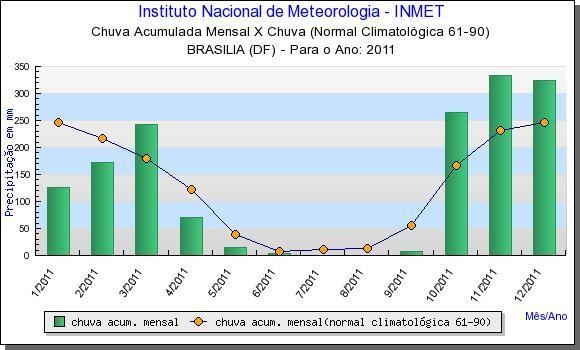
\includegraphics[scale=0.6]{captacao/1.jpg}
	 \caption{Chuva acumulada mensal (2011) x chuva (Normal climatólogia 61-90)\cite{INMET}.}
\end{figure}
 
 
\begin{figure}[H]
	 \centering
	\label{Chuva acumulada mensal (2012) x chuva (Normal climatólogia 61-90)}
	 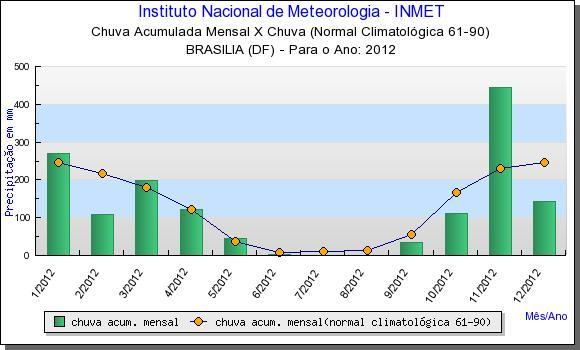
\includegraphics[scale=0.6]{captacao/2.jpg}
	 \caption{Chuva acumulada mensal (2012) x chuva (Normal climatólogia 61-90)\cite{INMET}.}
\end{figure}

\begin{figure}[H]
	 \centering
	\label{Chuva acumulada mensal (2013) x chuva (Normal climatólogia 61-90)}
	 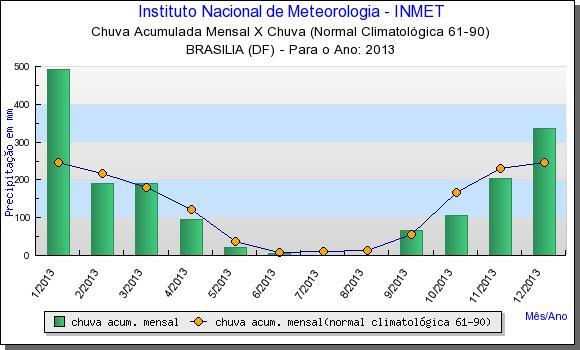
\includegraphics[scale=0.6]{captacao/3.jpg}
	 \caption{Chuva acumulada mensal (2011) x chuva (Normal climatólogia 61-90)\cite{INMET}.}
\end{figure}
 
 
\begin{figure}[H]
	 \centering
	\label{Chuva acumulada mensal (2014) x chuva (Normal climatólogia 61-90)}
	 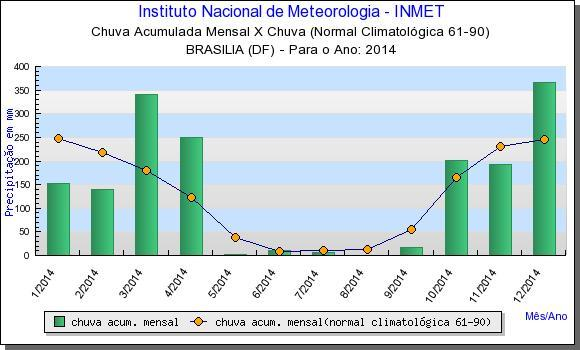
\includegraphics[scale=0.6]{captacao/4.jpg}
	 \caption{Chuva acumulada mensal (2012) x chuva (Normal climatólogia 61-90)\cite{INMET}.}
\end{figure}

\begin{table}[h]
\centering
\caption{Volume acumulado dos meses favoráveis a captação de água no DF (2011-2014) e (61-90).}
\label{Volume acumulado dos meses favoráveis a captação de água no DF (2011-2014) e (61-90).}
\begin{tabular}{llllll}
 &  &  &  &  &  \\ \hline
\multicolumn{1}{|l|}{} & \multicolumn{5}{l|}{Volume Acumulado em Litros} \\ \hline
\multicolumn{1}{|l|}{Mês} & \multicolumn{1}{l|}{2011} & \multicolumn{1}{l|}{2012} & \multicolumn{1}{l|}{2013} & \multicolumn{1}{l|}{2014} & \multicolumn{1}{l|}{Normal Clim. (61-90)} \\ \hline
\multicolumn{1}{|l|}{Janeiro} & \multicolumn{1}{l|}{49.072} & \multicolumn{1}{l|}{101.919,60} & \multicolumn{1}{l|}{186.852,60} & \multicolumn{1}{l|}{56.622} & \multicolumn{1}{l|}{94.370} \\ \hline
\multicolumn{1}{|l|}{Fevereiro} & \multicolumn{1}{l|}{64.171,60} & \multicolumn{1}{l|}{41.522,80} & \multicolumn{1}{l|}{71.721,20} & \multicolumn{1}{l|}{52.847,20} & \multicolumn{1}{l|}{83.045,60} \\ \hline
\multicolumn{1}{|l|}{Março} & \multicolumn{1}{l|}{90.595,20} & \multicolumn{1}{l|}{75.496} & \multicolumn{1}{l|}{71.721,20} & \multicolumn{1}{l|}{128.343,20} & \multicolumn{1}{l|}{67946,4} \\ \hline
\multicolumn{1}{|l|}{Abril} & \multicolumn{1}{l|}{26.423,60} & \multicolumn{1}{l|}{45.297,60} & \multicolumn{1}{l|}{33.973,20} & \multicolumn{1}{l|}{94.370} & \multicolumn{1}{l|}{49.072,40} \\ \hline
\multicolumn{1}{|l|}{Outubro} & \multicolumn{1}{l|}{101.919,60} & \multicolumn{1}{l|}{37.748} & \multicolumn{1}{l|}{37.748} & \multicolumn{1}{l|}{75.496} & \multicolumn{1}{l|}{64.171,60} \\ \hline
\multicolumn{1}{|l|}{Novembro} & \multicolumn{1}{l|}{124.568,40} & \multicolumn{1}{l|}{166.091,20} & \multicolumn{1}{l|}{75.496} & \multicolumn{1}{l|}{71.721,20} & \multicolumn{1}{l|}{86.820,40} \\ \hline
\multicolumn{1}{|l|}{Dezembro} & \multicolumn{1}{l|}{120.793,60} & \multicolumn{1}{l|}{52.847,20} & \multicolumn{1}{l|}{128.343,20} & \multicolumn{1}{l|}{139.667,60} & \multicolumn{1}{l|}{90.595,20} \\ \hline
\multicolumn{1}{|l|}{TOTAL} & \multicolumn{1}{l|}{577.544} & \multicolumn{1}{l|}{520.922,40} & \multicolumn{1}{l|}{605.855,40} & \multicolumn{1}{l|}{619.067,20} & \multicolumn{1}{l|}{536.021,60} \\ \hline
\end{tabular}
\end{table}

	Após calculado o quanto de água da chuva os telhados do Parque Urbano e Vivencial do Gama coletaram mensalmente e o acumulado para os meses favoráveis a captação da água da chuva no Distrito Federal durante os anos de 2011 e 2014. Agora é preciso determinar o quanto o Parque Urbano e Vivencial do Gama gastará em litros com o uso de descargas e irrigação de jardins.  
	
\subsection{Uso de descargas}

	Após calculado o quanto de água da chuva os telhados do Parque Urbano e Vivencial do Gama coletaram mensalmente e o acumulado para os meses favoráveis a captação da água da chuva no Distrito Federal durante os anos de 2011 e 2014. Agora é preciso determinar o quanto o Parque Urbano e Vivencial do Gama gastará em litros com o uso de descargas e irrigação de jardins.  
	Espera-se que após o témino das obras no Parque Urbano e Vivencial do Gama o parque receba em torno de 1300 pessoas em dias cheios. Estimando que o parque receba 3000 pessoas por semana e que a descarga dos banheiros sejam utilizadas 1500 vezes e que em cada descarga sejam gastos 6L como no que será utilizado no PUVG - Vaso Sanitário com Caixa Acoplada 3/6L Azálea Branco. Deve-se considerar também que a seca no Distrito Federal dura 5 a 6 meses, portanto a estimativa deve incluí-los. 
	
\begin{table}[h]
\centering
\caption{Consumo total de água em descarga do PUVG nos 6 meses de seca no DF.}
\label{Consumo total de água em descarga do PUVG nos 6 meses de seca no DF.}
\begin{tabular}{lllll}
 &  &  &  &  \\ \hline
\multicolumn{1}{|l|}{Nº descargas/Semana} & \multicolumn{1}{l|}{Litros/Descarga} & \multicolumn{1}{l|}{Dias} & \multicolumn{1}{l|}{Meses} & \multicolumn{1}{l|}{TOTAL em litros} \\ \hline
\multicolumn{1}{|l|}{1500} & \multicolumn{1}{l|}{6} & \multicolumn{1}{l|}{30} & \multicolumn{1}{l|}{6} & \multicolumn{1}{l|}{216.000} \\ \hline
\multicolumn{1}{|l|}{2000} & \multicolumn{1}{l|}{6} & \multicolumn{1}{l|}{30} & \multicolumn{1}{l|}{6} & \multicolumn{1}{l|}{360.000} \\ \hline
\end{tabular}
\end{table}

Portanto, caso em determinado ano a seca se prolongue por 6 meses (normalmente são 5) o parque consumirá de 216.000 L a 360.000 L, quando realizadas 1500 e 2000 descargas por semana respectivamente. 

\subsection{Quanto eu consigo captar?}

Analisando a tabela 14, especificamente a coluna da Normal Climatológica que revela que o quanto o Parque consegue coletar em litros de água com a superfície de 377,48m2 (área telhados do parque), obtêm-se o valor de 536.021,6L. É baseado nesse valor que se fará o dimensionamento do sistema. Pois a estrutura utilizada para o reservatório (Cement Plate Cistern) comporta até 20 mil litros cada \cite{gnadlinger1999technical}. Logo, seria preciso 27 dessas ou reservatórios maiores ao redor das instalações do parque. No entanto, serão utilizados 8 tanques com capacidade total de 160.000L. Como a água dos reservatórios será utilizada também no período em que está sendo captada e o parque consume mensalmente 60.000L, nem todos os meses a água armazenada será consumida. A tabela abaixo mostra o quanto o parque consegue captar, o volume de água consumida mensalmente (descargas) e o quanto da água captada mensalmente sobraria.

\begin{table}[h]
\centering
\caption{Volume Residual Mensal.}
\label{Volume Residual Mensal.}
\begin{tabular}{lccc}
 & \multicolumn{1}{l}{} & \multicolumn{1}{l}{} & \multicolumn{1}{l}{} \\ \hline
\multicolumn{4}{|c|}{Volume Residual Mensal} \\ \hline
\multicolumn{1}{|l|}{Mês} & \multicolumn{1}{l|}{Volume Captado Mensalmente (Norm. Clim.)} & \multicolumn{1}{l|}{Volume Consumido Mensalmente} & \multicolumn{1}{l|}{Volume Residual em L} \\ \hline
\multicolumn{1}{|l|}{Janeiro} & \multicolumn{1}{c|}{94.370} & \multicolumn{1}{c|}{60.000L} & \multicolumn{1}{c|}{34.370} \\ \hline
\multicolumn{1}{|l|}{Fevereiro} & \multicolumn{1}{c|}{83.045,60} & \multicolumn{1}{c|}{60.000L} & \multicolumn{1}{c|}{23.045,60} \\ \hline
\multicolumn{1}{|l|}{Março} & \multicolumn{1}{c|}{67946,4} & \multicolumn{1}{c|}{60.000L} & \multicolumn{1}{c|}{7.946,40} \\ \hline
\multicolumn{1}{|l|}{Abril} & \multicolumn{1}{c|}{49.072,40} & \multicolumn{1}{c|}{60.000L} & \multicolumn{1}{c|}{-10.927,60} \\ \hline
\multicolumn{1}{|l|}{Outubro} & \multicolumn{1}{c|}{64.171,60} & \multicolumn{1}{c|}{60.000L} & \multicolumn{1}{c|}{4.171,60} \\ \hline
\multicolumn{1}{|l|}{Novembro} & \multicolumn{1}{c|}{86.820,40} & \multicolumn{1}{c|}{60.000L} & \multicolumn{1}{c|}{26.820,40} \\ \hline
\multicolumn{1}{|l|}{Dezembro} & \multicolumn{1}{c|}{90.595,20} & \multicolumn{1}{c|}{60.000L} & \multicolumn{1}{c|}{30.595,20} \\ \hline
\end{tabular}
\end{table}

Como a captação será feita durante sete meses, quando começar o período de estiagem a partir de maio e que segue por cinco meses, o reservatório terá acumulado em água 116.949,2L pois é preciso levar em conta que no mês de abril o volume residual foi negativo. Esse volume residual é quase suficiente para abastecer o parque por mais dois meses, sendo assim durante apenas três o consumo seria suprido pela companhia de abastecimento do Distrito Federal (CAESB).

\subsection{Processo de captação}

No processo de captação da água, são utilizadas áreas impermeáveis, como por exemplo nos telhados. Este projeto visa a disponibilização da coleta da água nos telhados dos banheiros, da administração e das torres de segurança. Nos locais que tiver certa inclinação, serão colocadas calhas capazes de canalizar a água e levá-la para os tanques, onde serão tratadas e enviadas para sua utilização \cite{MAY}.

Segundo a Leal \cite{LEAL} , o sistema de aproveitamento da água da chuva funciona da seguinte maneira: a água é coletada de áreas impermeáveis e em seguida é filtrada e armazenada em um reservatório de acumulação, que pode ser apoiado, enterrado ou elevado e pode ser construído de diferentes materiais como: concreto armado, bloco de concreto, alvenaria de tijolos, aço, plástico, poliéster, polietileno e outros. 

Os parâmetros principais envolvidos no sistema de coleta e aproveitamento da água de chuva são: área de coleta, quantidade de água a ser armazenada, qualidade da água, capacidade de armazenamento e confiabilidade. 
Para não ocorrerem entupimentos nos dutos que levam a água canalizada para os tanques são usadas peneiras para retirada de folhas e galhos maiores, essas grades serão posicionadas por toda a calha aumentando um pouco o custo, porém evitando possíveis problemas na filtragem, como pode ser observado na Figura 1. Será usado 122mm x 3m dessa calha, e pode ser encontrada na  Leroy Merlin a um valor de R\$ 59,90.

\begin{figure}[H]
	 \centering
	\label{Grades usada na calha.}
	 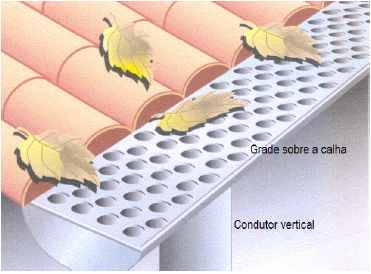
\includegraphics[scale=0.6]{captacao/5.png}
	 \caption{Grades usada na calha \cite{WATERFALL}.}
\end{figure}

\begin{figure}[H]
	 \centering
	\label{Sistema de calhas na área do telhado.}
	 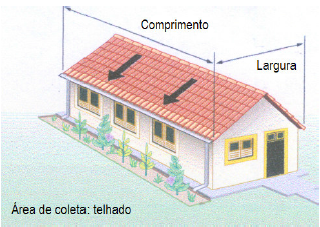
\includegraphics[scale=0.6]{captacao/6.png}
	 \caption{Sistema de calhas na área do telhado \cite{WATERFALL}.}
\end{figure}

O armazenamento será feito a partir do estudo de 8 tipos de tanques, devido a disponibilidade e a facilidade de construção, para tanto foi realizado um estudo, apresentado na Figura 115, da capacidade de armazenamento, viabilidade econômica, e mão-de-obra.

\begin{figure}[H]
	 \centering
	\label{Tipo de Tanques}
	 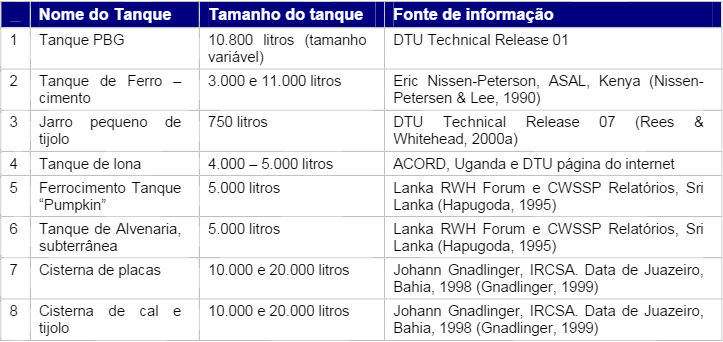
\includegraphics[scale=0.6]{captacao/7.png}
	 \caption{Tipo de Tanques \cite{gnadlinger1999technical}.}
\end{figure}

\begin{figure}[H]
	 \centering
	\label{Comparativo dos tanques}
	 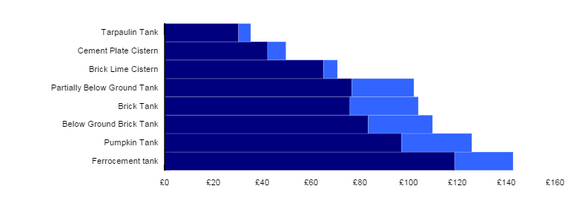
\includegraphics[scale=0.6]{captacao/8.png}
	 \caption{Comparativo dos tanques \cite{gnadlinger1999technical}.}
\end{figure}

O gráfico da figura 116 foi feito a partir das informções da Figura 115 sobre os tipos de tanques, mostrando o custo do material, a conversão foi feita seguindo a cotação atual, sendo 1 libra esterlina 4,36 reais.

Tendo em vista os tanques estudados na e apresentados na Figura 115, o que se mostrou mais economicamente atrativo foi o “Cement Plate Cistern”, a cisterna de placas cimentadas, a qual armazena de 10 mil a 20 mil litros de água, o mesmo é melhor para o parque devido ao seu custo de operação e instalação serem baixos, o cimento é barato, gerando um custo de 500 reais para a construção. O tanque do tipo placas cimentadas segue a ideia de ser encostado na edificação, portanto eles serão posicionados ao lado dos banheiros, guarita de segurança, administração e quiosque sem consumir muito espaço e com sinalização para que os usuários não mexam na instalação. A Figura 117 apresenta o sistema de captação de água a ser implantado no Parque do Gama \cite{gnadlinger1999technical}. 

\begin{figure}[H]
	 \centering
	\label{sistema de captação}
	 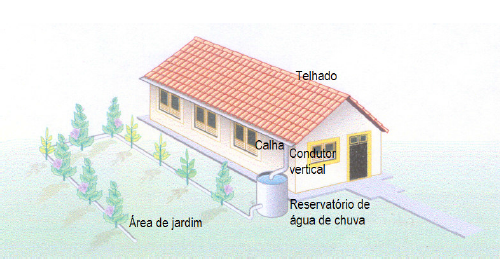
\includegraphics[scale=0.6]{captacao/9.png}
	 \caption{sistema de captação \cite{WATERFALL}.}
\end{figure}

Um ponto relevante a ser considerado é que em hipótese alguma a água de chuva captada poderá ser misturada a água potável. Ademais, é necessário que haja limpeza da água. Para realizar a limpeza da água, será usado um filtro VF1 o qual recebe a água da chuva e filtra os galhos e folhas que passaram pela grade das calhas, em seguida, a água da chuva passa por uma tela de malha de 0,26mm que se localiza abaixo das ripas e é direcionada ao reservatório. A frequência da manutenção varia conforme a incidência da sujeira, ocorrendo de 1 a 2 vezes ao ano. O filtro, o qual vai ser utilizado, é mostrado na Figura 119 e pode ser encontrado no valor de 2100 reais. 


\begin{figure}[H]
	 \centering
	\label{Sistema de filtro utilizado}
	 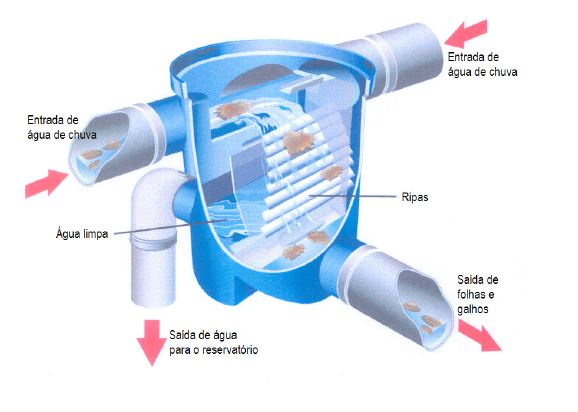
\includegraphics[scale=0.6]{captacao/10.png}
	 \caption{Sistema de filtro utilizado \cite{ECOCASA} .}
\end{figure}

A tabela 6 apresenta o tipo da água da chuva, com o filtro usado e a desinfecção requerida, no parque será utilizada água não potável, pois apresenta filtros e tratamento químico com cloro, para no caso de contato com a pele, não cause nenhum efeito colateral.

\begin{table}[h]
\centering
\caption{tipo da agua e propriedades exigidas.}
\label{tipo da agua e propriedades exigidas}
\begin{tabular}{llll}
 &  &  &  \\ \hline
\multicolumn{1}{|l|}{} & \multicolumn{3}{l|}{Aplicações Básicas} \\ \hline
\multicolumn{1}{|l|}{Tratamento necessário} & \multicolumn{1}{l|}{Potável} & \multicolumn{1}{l|}{Não potável} & \multicolumn{1}{l|}{Rega e Limpeza} \\ \hline
\multicolumn{1}{|l|}{\begin{tabular}[c]{@{}l@{}}Filtros a serem\\  instalados\end{tabular}} & \multicolumn{1}{l|}{\begin{tabular}[c]{@{}l@{}}Filtro para sedimentos e no \\ mínimo outro de carvão \\ ativado, para eliminar \\ produtos químicos.\end{tabular}} & \multicolumn{1}{l|}{\begin{tabular}[c]{@{}l@{}}Filtro de sedimentos e \\ partículas alem de \\ tratamento com cloro.\end{tabular}} & \multicolumn{1}{l|}{\begin{tabular}[c]{@{}l@{}}É suficiente um filtro por \\ gravidade de pedras.\end{tabular}} \\ \hline
\multicolumn{1}{|l|}{Desinfecção requerida} & \multicolumn{1}{l|}{Necessário/fundamental} & \multicolumn{1}{l|}{Necessário} & \multicolumn{1}{l|}{Não é necessária} \\ \hline
\end{tabular}
\end{table}

A qualidade da água é definida pela sua composição física, química e bacteriológica. Como a água da chuva captada não será direcionada para o consumo ela não precisa ser potável, portanto o tratamento necessário para ela é um cuidado com bactérias capazes de criar enfermidades ou qualquer organismo capazes de provocar enfermidades. \cite{sorgato2014analise}  Mesmo a água não sendo utilizada para o consumo ela deve ser corretamente tratada por entrar em contato com os seres humanos na irrigação, nas descargas do banheiro ou na limpeza, não podendo, então, conter bactérias causadoras de enfermidades.

A desinfecção de água de chuva poderá ser realizada através de sistema simples, como através de adição de cloro, para não inviabilizar economicamente o sistema. O cloro deverá ser aplicado de forma mais homogênea possível, devendo repetir a operação sempre que o teor de cloro ficar muito baixo alem de não alterar no pH da água. A desinfecção é um tratamento prioritário porque se uma água não for bem tratada e podendo estar contaminada poderá trazer sérios riscos à saúde. O preço do cloro é relativamente baixo, de em torno de 150 reais o pote de 10 kg.

Para bombeamento da água será utilizado uma bomba d’água acoplada a rede elétrica monofásica submersa de ¾ de polegada que utiliza 300 watts e 220v ECCO - Anauger por ter um preço baixo, de aproximadamente 200 reais no mercado, com excelente vazão com pressão que alcança bombeamento de altura máxima de 50 metros.

O sistema de captação de água reduzirá notavelmente o consumo total de água do parque, e nos períodos de seca, essa água armazenada poderá ser devidamente utilizada para irrigação dos jardins próximos à área do banheiro, além de servir para o uso em descargas e limpeza dos pisos. O reuso da água da chuva que será instalado é um ótimo caminho para tornar o parque em um parque modelo de sustentabilidade.

Dessa forma, o custo de construção girará em torno de 4300 reais por local de instalação, contando com a mão-de-obra e com os materiais, e para a manutenção foi estipulado um valor de 200 reais por mês para mão de obra e purificação da água, assim em aproximadamente um ano a água economizada com a instalação desse sistema de captação cobrirá os custos iniciais, levando em consideração a quantidade de pessoas que frequentarão o parque e a quantidade de chuvas que pode variar a cada ano.

\subsection{Quanto custa o $M^{3}$ da CAESB?}

O parque mensalmente irá consumir:
\begin{itemize}
	\item 60.000L de água em descargas (60 $m^{2}$);
\end{itemize}

	
	Tendo em vista que durante 3 meses o abastecimento será feito pela companhia de abastecimento do DF. Calculando quanto o parque teria que pagar a CAESB em tributos mensalmente, utilizando as tarifas atualmente vigentes na companhia obtêm-se: 
	
\begin{table}[h]
\centering
\caption{Valor pago mensalmente a CAESB (estimativa)}
\label{Valor pago mensalmente a CAESB (estimativa)}
\begin{tabular}{lllll}
 &  &  &  &  \\ \hline
\multicolumn{1}{|l|}{Uso} & \multicolumn{1}{l|}{Consumo Mensal em L} & \multicolumn{1}{l|}{M3} & \multicolumn{1}{l|}{Tarifa} & \multicolumn{1}{l|}{Custo em Reais} \\ \hline
\multicolumn{1}{|l|}{Descargas} & \multicolumn{1}{l|}{60.000} & \multicolumn{1}{l|}{60} & \multicolumn{1}{l|}{10,82 (\textgreater10 $m{3}$)} & \multicolumn{1}{l|}{649,2} \\ \hline
\multicolumn{1}{|l|}{TOTAL} & \multicolumn{1}{l|}{} & \multicolumn{1}{l|}{} & \multicolumn{1}{l|}{} & \multicolumn{1}{l|}{649,20 BRL} \\ \hline
\end{tabular}
\end{table}

Mensalmente a administração do Parque Urbano e Vivencial do Gama gastaria R\$ 649,20 reais em conta de água e nos outros 3 meses onde será utilizada água pública R\$ 1.947,60 reais. Caso o parque fosse pagar pelos seus 720m3 utilizados anualmente essa conta seria de R\$ 7.790,40 que deveriam ser pagos a CAESB. Entretanto, como o parque gasta apenas R\$ 1.947,60 em tributos à CAESB, a economia acaba sendo de R\$ 5.842,80 anualmente em conta de água. 
